\documentclass[a4paper]{article}
\usepackage{enumerate} %Let's us specify how to number enumerations
\usepackage{fullpage}  %Make the margins a bit smaller (not always sensible...)
\usepackage{graphicx}  %Ensures that \includegraphics will work
\usepackage{framed}
\usepackage{amsmath}
\usepackage{amsfonts}
\usepackage{bbm}
\usepackage{listings}
\usepackage{color}
\usepackage{amssymb}

%You may also find the listings package useful for including sourcecode
 

\begin{document}
\title{Network Analytics}
\author{\bf Group 4}
\maketitle
\section*{Question 1}

\begin{enumerate}[(a)]
\item \textbf{Incidence Matrix}

We read the data into using the \texttt{read\_edgelist()} function and get the following incidence matrix.
\begin{table}[ht]
\begin{center}
\begin{tabular}{c|cccccccc}
& (a,b) & (a,d) & (d,b) & (d,e) & (b,e) &(b,c) & (c,d)\\
\hline
a & -1 & -1 	& 0 	& 0 	& 0	& 0	&0\\
b &1 	& 0	& 1 	& 0	& -1	& -1	& 0\\
c &0 	& 0 	& 0 	& 0	&0	&1	&-1\\
d & 0 	& 1 	& -1 	& -1	& 0	&0	&1\\
e & 0 	& 0 	& 0 	& 1	& 1	&0	&0\\
\end{tabular}
\end{center}
\end{table}

\item \textbf{Shortest Path Matrix}

\begin{table}[ht]
\begin{center}
\begin{tabular}{c|cccccccc}
& a & b & c & d & e\\
\hline
a & 0 		& 5	& 15	& 3 	& 6\\
b &$\inf$ 	& 0	& 10 	& 8	& 7\\
c &$\inf$ 	& 6 	& 0 	& -2	& 1\\
d &$\inf$ 	& 8 	& 18 	& 0	& 3\\
e &$\inf$ 	&$\inf$& $\inf$& $\inf$	& 0
\end{tabular}
\end{center}
\end{table}

\item \textbf{Diameter}

Using the shortest path matrix above, we iterate through all values to find the maximum value while ignoring the $\infty$ values. The diameter of the graph is 18.

\item \textbf{Degree Distribution}

\begin{center}
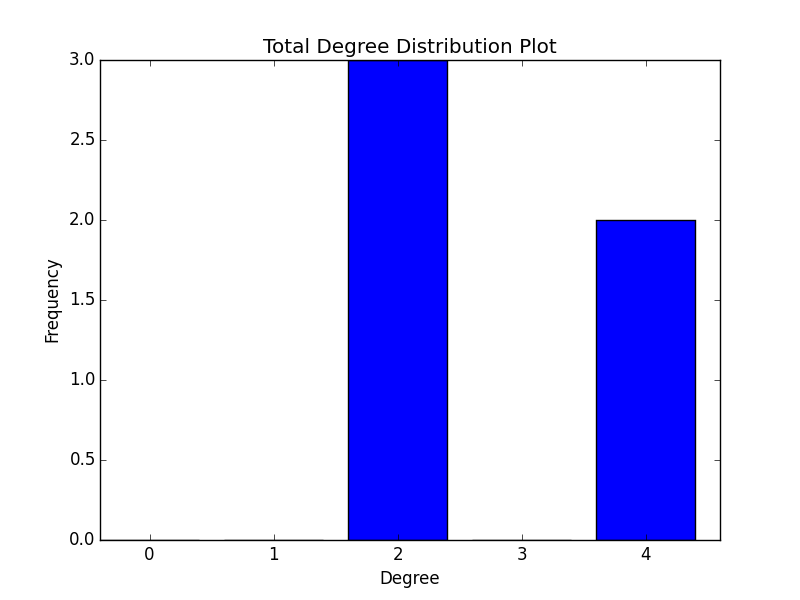
\includegraphics[width=100mm]{degree_histogram.png}
\end{center}

The support of the distribution is \{2,4\} with the probabilities,

$$\mathbb{P}(K=k)=
\begin{cases}
\frac{3}{5}, \text{if }k=2\\
\frac{2}{5}, \text{if }k=4
\end{cases}
$$

\item \textbf{Connectedness}

Using the commands \texttt{print(nx.is\_strongly\_connected(G))} and \texttt{print(nx.is\_weakly\_connected(G))}, we check both weak and strong connectivity. We find that the graph is WEAKLY connected but not STRONGLY connected due to the directed edges.

\end{enumerate}

\section*{Question 2}

\begin{center}
\includegraphics[width=\linewidth]{graph_plot.png}
\end{center}

Because all of the nodes in the graph are somewhat connected with each other, when drawing the graph, it is important to visualize it in a way that shows which nodes are connected with each other, placing nodes in their relative places to each other. The Fruchterman Reingold format for the graph shows that nodes 0, 32, and 33 in particular have high degrees and thus are considered as nodes towards the center. In a similar manner, nodes with low degrees are plotted towards the outside of the graph, which makes it easy to visualize a node's relation to other nodes. Therefore the Fruchterman Reingold layout displays a graph that displays a node's degree well in addition to visualizing the edges between nodes without much overlap. The visualization combines the adjacency matrix to draw the presence of an edge, and also displays the edge's weight. Thus, the algorithm provides a balance between emphasizing a graph's connectedness, adjacency, edge weights, and node degrees.

\end{document}
